\documentclass{standalone}
\usepackage{tikz}
\usetikzlibrary{patterns, positioning}


\begin{document}
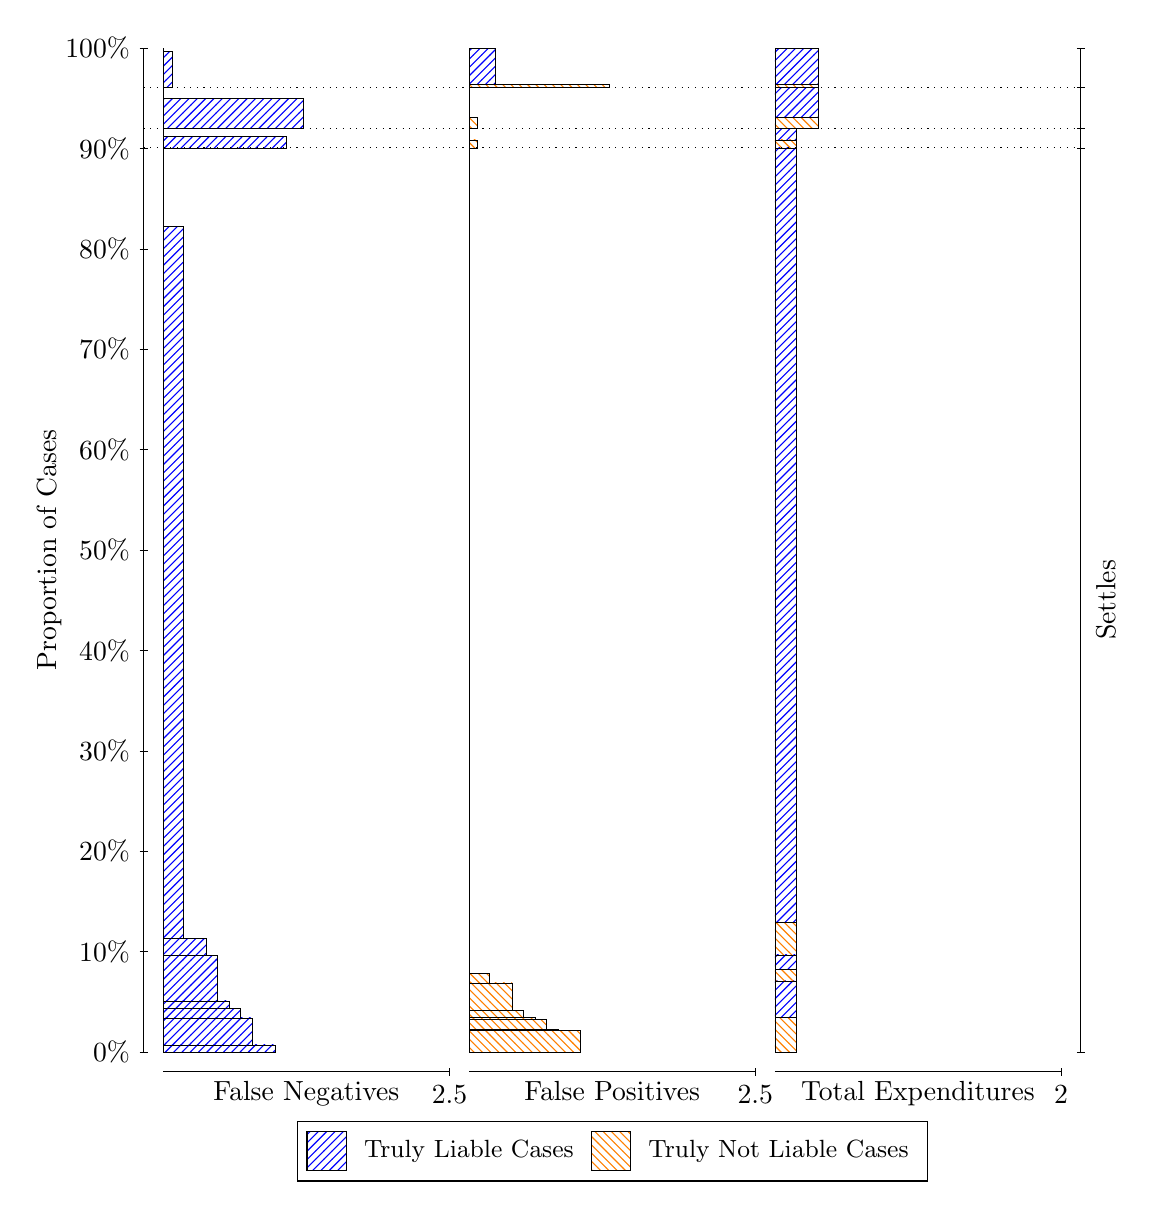
\begin{tikzpicture}
\draw[black, very thin] (1.5,1.75) -- (1.5,14.5);
\node[rotate=90, text=black, anchor=center] at (0.3, 8.125) {Proportion of Cases};
\draw[black, very thin] (1.45,1.75) -- (1.55,1.75);
\node[text=black, anchor=east] at (1.45, 1.75) {0\%};
\draw[black, very thin] (1.45,3.025) -- (1.55,3.025);
\node[text=black, anchor=east] at (1.45, 3.025) {10\%};
\draw[black, very thin] (1.45,4.3) -- (1.55,4.3);
\node[text=black, anchor=east] at (1.45, 4.3) {20\%};
\draw[black, very thin] (1.45,5.575) -- (1.55,5.575);
\node[text=black, anchor=east] at (1.45, 5.575) {30\%};
\draw[black, very thin] (1.45,6.85) -- (1.55,6.85);
\node[text=black, anchor=east] at (1.45, 6.85) {40\%};
\draw[black, very thin] (1.45,8.125) -- (1.55,8.125);
\node[text=black, anchor=east] at (1.45, 8.125) {50\%};
\draw[black, very thin] (1.45,9.4) -- (1.55,9.4);
\node[text=black, anchor=east] at (1.45, 9.4) {60\%};
\draw[black, very thin] (1.45,10.675) -- (1.55,10.675);
\node[text=black, anchor=east] at (1.45, 10.675) {70\%};
\draw[black, very thin] (1.45,11.95) -- (1.55,11.95);
\node[text=black, anchor=east] at (1.45, 11.95) {80\%};
\draw[black, very thin] (1.45,13.225) -- (1.55,13.225);
\node[text=black, anchor=east] at (1.45, 13.225) {90\%};
\draw[black, very thin] (1.45,14.5) -- (1.55,14.5);
\node[text=black, anchor=east] at (1.45, 14.5) {100\%};

\draw[black, very thin] (13.4,1.75) -- (13.4,14.5);
\draw[black, very thin] (13.35,1.75) -- (13.45,1.75);
\node[anchor=west] at (13.35, 1.75) {};
\draw[black, very thin] (13.35,13.233) -- (13.45,13.233);
\node[anchor=west] at (13.35, 13.233) {};
\draw[black, very thin] (13.35,13.477) -- (13.45,13.477);
\node[anchor=west] at (13.35, 13.477) {};
\draw[black, very thin] (13.35,13.998) -- (13.45,13.998);
\node[anchor=west] at (13.35, 13.998) {};
\draw[black, very thin] (13.35,14.5) -- (13.45,14.5);
\node[anchor=west] at (13.35, 14.5) {};

\draw[black, very thin, pattern color=blue, pattern=north east lines] (1.75,1.75) rectangle (3.167,1.8399);
\draw[black, very thin, pattern color=blue, pattern=north east lines] (1.75,1.8399) rectangle (2.8763,2.1833);
\draw[black, very thin, pattern color=blue, pattern=north east lines] (1.75,2.1833) rectangle (2.731,2.3064);
\draw[black, very thin, pattern color=blue, pattern=north east lines] (1.75,2.3064) rectangle (2.5857,2.3979);
\draw[black, very thin, pattern color=blue, pattern=north east lines] (1.75,2.3979) rectangle (2.4403,2.9807);
\draw[black, very thin, pattern color=blue, pattern=north east lines] (1.75,2.9807) rectangle (2.295,3.1898);
\draw[black, very thin, pattern color=blue, pattern=north east lines] (1.75,3.1898) rectangle (2.0043,12.239);
\draw[black, very thin, pattern color=orange, pattern=north west lines] (1.75,12.239) rectangle (1.75,13.233);
\draw[black, very thin, pattern color=blue, pattern=north east lines] (1.75,13.233) rectangle (3.3123,13.376);
\draw[black, very thin, pattern color=orange, pattern=north west lines] (1.75,13.376) rectangle (1.75,13.477);
\draw[black, very thin, pattern color=blue, pattern=north east lines] (1.75,13.477) rectangle (3.5303,13.86);
\draw[black, very thin, pattern color=orange, pattern=north west lines] (1.75,13.86) rectangle (1.75,13.998);
\draw[black, very thin, pattern color=blue, pattern=north east lines] (1.75,13.998) rectangle (1.859,14.458);
\draw[black, very thin, pattern color=orange, pattern=north west lines] (1.75,14.458) rectangle (1.75,14.5);
\draw[black, very thin, pattern color=orange, pattern=north west lines] (5.6333,1.75) rectangle (7.0503,2.0205);
\draw[black, very thin, pattern color=orange, pattern=north west lines] (5.6333,2.0205) rectangle (6.7597,2.0337);
\draw[black, very thin, pattern color=orange, pattern=north west lines] (5.6333,2.0337) rectangle (6.6143,2.1593);
\draw[black, very thin, pattern color=orange, pattern=north west lines] (5.6333,2.1593) rectangle (6.469,2.1916);
\draw[black, very thin, pattern color=orange, pattern=north west lines] (5.6333,2.1916) rectangle (6.3237,2.278);
\draw[black, very thin, pattern color=orange, pattern=north west lines] (5.6333,2.278) rectangle (6.1783,2.6267);
\draw[black, very thin, pattern color=orange, pattern=north west lines] (5.6333,2.6267) rectangle (5.8877,2.7437);
\draw[black, very thin, pattern color=blue, pattern=north east lines] (5.6333,2.7437) rectangle (5.6333,13.233);
\draw[black, very thin, pattern color=orange, pattern=north west lines] (5.6333,13.233) rectangle (5.7423,13.333);
\draw[black, very thin, pattern color=blue, pattern=north east lines] (5.6333,13.333) rectangle (5.6333,13.477);
\draw[black, very thin, pattern color=orange, pattern=north west lines] (5.6333,13.477) rectangle (5.7423,13.615);
\draw[black, very thin, pattern color=blue, pattern=north east lines] (5.6333,13.615) rectangle (5.6333,13.998);
\draw[black, very thin, pattern color=orange, pattern=north west lines] (5.6333,13.998) rectangle (7.4137,14.04);
\draw[black, very thin, pattern color=blue, pattern=north east lines] (5.6333,14.04) rectangle (5.9603,14.5);
\draw[black, very thin, pattern color=orange, pattern=north west lines] (9.5167,1.75) rectangle (9.7892,2.1851);
\draw[black, very thin, pattern color=blue, pattern=north east lines] (9.5167,2.1851) rectangle (9.7892,2.6516);
\draw[black, very thin, pattern color=orange, pattern=north west lines] (9.5167,2.6516) rectangle (9.7892,2.8009);
\draw[black, very thin, pattern color=blue, pattern=north east lines] (9.5167,2.8009) rectangle (9.7892,2.9823);
\draw[black, very thin, pattern color=orange, pattern=north west lines] (9.5167,2.9823) rectangle (9.7892,3.3915);
\draw[black, very thin, pattern color=blue, pattern=north east lines] (9.5167,3.3915) rectangle (9.7892,13.233);
\draw[black, very thin, pattern color=orange, pattern=north west lines] (9.5167,13.233) rectangle (9.7892,13.333);
\draw[black, very thin, pattern color=blue, pattern=north east lines] (9.5167,13.333) rectangle (9.7892,13.477);
\draw[black, very thin, pattern color=orange, pattern=north west lines] (9.5167,13.477) rectangle (10.062,13.615);
\draw[black, very thin, pattern color=blue, pattern=north east lines] (9.5167,13.615) rectangle (10.062,13.998);
\draw[black, very thin, pattern color=orange, pattern=north west lines] (9.5167,13.998) rectangle (10.062,14.04);
\draw[black, very thin, pattern color=blue, pattern=north east lines] (9.5167,14.04) rectangle (10.062,14.5);
\draw[black, dotted] (1.5,13.233) -- (13.4,13.233);
\draw[black, dotted] (1.5,13.477) -- (13.4,13.477);
\draw[black, dotted] (1.5,13.998) -- (13.4,13.998);
\draw[black, very thin] (1.75,1.5) -- (5.3833,1.5);
\node[text=black, anchor=north] at (3.5667, 1.5) {False Negatives};
\draw[black, very thin] (5.3833,1.45) -- (5.3833,1.55);
\node[text=black, anchor=north] at (5.3833, 1.45) {2.5};

\draw[black, very thin] (5.6333,1.5) -- (9.2667,1.5);
\node[text=black, anchor=north] at (7.45, 1.5) {False Positives};
\draw[black, very thin] (9.2667,1.45) -- (9.2667,1.55);
\node[text=black, anchor=north] at (9.2667, 1.45) {2.5};

\draw[black, very thin] (9.5167,1.5) -- (13.15,1.5);
\node[text=black, anchor=north] at (11.333, 1.5) {Total Expenditures};
\draw[black, very thin] (13.15,1.45) -- (13.15,1.55);
\node[text=black, anchor=north] at (13.15, 1.45) {2};

\node[text=black, centered, rotate=90] at (13.72, 7.4914) {Settles};




\draw (7.449999999999999,1.5) node[draw=none] (baseCoordinate) {};
\begin{scope}[align=center]
        \matrix[scale=0.5, draw=black, below=0.5cm of baseCoordinate, nodes={draw}, column sep=0.1cm]{
            \node[rectangle, draw, minimum width=0.5cm, minimum height=0.5cm, pattern color=blue, pattern=north east lines] {}; &
            \node[draw=none, font=\small, text=black] (B) {Truly Liable Cases}; &
            \node[rectangle, draw, minimum width=0.5cm, minimum height=0.5cm, pattern color=orange, pattern=north west lines] {}; &
            \node[draw=none, font=\small, text=black] (B) {Truly Not Liable Cases}; \\
            };
\end{scope}

\end{tikzpicture}
\end{document}